\documentclass[11pt]{article}
\usepackage[margin=1in]{geometry}
\usepackage[parfill]{parskip}
\usepackage{tabularx}
\usepackage{amsmath}
\usepackage{graphicx}

\title{DECINT WHITE PAPER}
\author{Christopher Rae \\ \begin{small} email: raecd123@gmail.com \end{small}}

\date{}

\newcommand{\textify}[1]{\text{\begin{scriptsize}#1\end{scriptsize}}}

\begin{document}
\maketitle

\tableofcontents
\newpage
\section{Introduction}

\section{Blocks} 
\subsection{Transactions}
Transaction on the DECINT blockchain use the SECP112r2 ecdsa encryption curve to sign transactions transaction are signed slightly differently depending on the transaction type. Currently there 3 different types of transaction the first being the normal token transfer transaction it looks like this:
\
\begin{center}
\{time: 1671020930.9900985,  sender: "...",  receiver: "...",  amount: 657.0,  sig: "..."\}
\end{center}

These types of transactions are made up of 5 parts. The time in Unix Time, the senders public key which consists of a 56 character string generated from the SECP112r2 curve, followed by the receivers public key, then the amount sent and finally the transaction signature the transaction signature is generate from a string of all the information in the transaction separated by a blank space " " and signed using the senders private key. All token transfer transactions have a 1\% transaction fee, 0.5\% of the transaction goes to the validator of the block which the transaction is in, the other 0.5\% is put towards the AI training nodes.  

The next 2 types are are pretty similar these are the stake and unstake transactions. Both have the same structure:

\begin{center}
\{time: 1671020930.9900985,  pub\_key: "...",  stake\_amount: 657.0,  sig: "..."\}
\end{center}

In the case of unstaking stake\_amount becomes unstake\_amount. the process of signing is the same as with token transfer transaction. There are no transaction fees associated with staking and unstaking.
\subsection{Temp Blocks}
Blocks are created based on time. As of writing, every transaction that happens within 2 minutes from the first transaction in a block is added to that block, the next transaction after that 2 minutes, acts as the first transaction in the next block and the process repeats. 

Temp blocks are made up of 3 parts the head, main body and tail. The head is a list of values the first being the hash of the previous temp block followed by the block index and the time of the first transaction in the block:

\begin{center}
["6db4f412053b48a7f2579ed59d28a7d623ef6ebc9d5023b17cb331b8b92d5be8", 2, 1802.9900985]
\end{center}

The main body is made up of all the transactions that occur within the time allocated for that block:

\begin{center}
[[HEAD], \{"time": 1802.9900985, "pub\_key": "...", "stake\_amount": 1.0, "sig": "..."\},\\          \hspace{0.75cm}\{time: 1850.23739823,  pub\_key: "...",  stake\_amount: 657.0,  sig: "..."\}]
\end{center}

The tail is added when the next block is created, it is made up of 3 parts.The first holds the blocks hash and the time of the first transaction of the next block. The hash is calculated by concatenating all the signatures and the hash of the previous block into one long string. The second part is the total transaction fees rewarded for validating that block and the final part has 2 values a False boolean value to indicate that the block has not been validated and the time of the first transaction of the next block
 
\begin{center}
[[HEAD], TRANS, \\\hspace{0cm}["0a5d31b6e2c57dc6c81bf916006bd2c412eb79b3cedad7d90ec7a50ab2eeb78b", 1950.23791313], [6.57], [false, 1950.23791313]]
\end{center}

\subsection{Chain Block}
The chain block is the most important block when a block is validated it get added to the chain block. Much like the temp block the chain block also is made up of a head a main body and a tail, the head is the same as the temp block the main body however is made up of a json object where the keys are wallets. All transaction recorded in the temp block effect the values stored in the wallet(If the transaction is valid), so if Bob has 100 DCNT and send 20 to Alice, Bobs wallet value would go down by 20 and Alice's wallet would go up by 19.8 and the other 0.2 would be split between the validator and the AI nodes. If Bob staked 20 of his DCNT, his wallet would go down by 20. Instead of storing every transaction the nodes only store the current wallet values. 

The Tail is once again made up of 3 parts the first 2 not changing from the temp block but the 3rd part now contains 3 values the first being a True boolean value, the second being the time of validation and the third being the validators public key. The wallet value of the validator increase by the validation reward of the block within the main body of the block.



\section{Validation}
\subsection{Validator}
The Validator of a temp block is determined by the hash of the previous block (which is stored in the head of the block). Validation can only occur when the previous block has been validated in order for all nodes to share the same block hashes. The hexadecimal hash is converted into base-10 and used as the seed for the random algorithm. If a validator fails to validate within 20 seconds of the blocks tail being added, the next validator is chosen. This is done by generating the next node in the sequence based of the seed (the previous blocks hash), If that node then doesn't validate within the next 20 seconds the process repeats until the block is validated. If a node fails to validate within the allocated 20 seconds it will lose all the DCNT which it has staked and the node and any future node with the node's wallet will not be allowed to validate.

Each node has a weighted value associated with it dependent on how much has been stake it is scaled linearly. There is a minimum stake amount this is in place to discourage malicious nodes but there are plans to add built in staking pools for users who want to stake without the large upfront cost and running the risk of sending their DCNT to someone else's wallet.
\subsection{Validating Blocks}
When a transaction is received its time and signature are verified and it is added to the temp block. When validating a validator checks if every transaction to make sure it has the balance to make the requested transaction, if the transaction is true it adds it to a list of true transactions. The list of true transactions gets sent to every node, each node then checks every transaction if it agrees with all the transactions the main body of the chain block is updated with the new balances from, the transaction that occurred in the list of true transactions. If any of the transactions received in list of true transactions is false the validator will lose all the DCNT which it has staked and the node and any future node with the node's wallet will not be allowed to validate.

If a transaction is not received by the validator it will not be added to the chain block even if another node receives it. Once a block has been deemed valid its temp block is removed from the chain and the chain block is updated. All staking and unstaking transaction are saved with the block index in which they occurred in separate file.

\section{Communication}
\subsection{Structure}
TCP is used to communicate messages, which are encoded in UTF-8. All messages are communicated as a string. Each message starts with the protocol and is followed by the information for that protocol. Different Protocols contain different information for example a transaction message contains the time, sender, receiver, amount sent and the signature. Each element of the message is separate with with a space (" "):

\begin{center}
TRANS\hspace{0.1cm} 1802.9900985 \hspace{0.1cm} ae32... \hspace{0.1cm} 5687... \hspace{0.1cm}  679.0 \hspace{0.1cm} b34d...
\end{center}

It is important to make sure spaces are removed if sending a json object:

\begin{center}
"[{"a":12,"b":34,"c":-3},12]" $\neq$ "[{"a":12, "b":34, "c":-3}, 12]"
\end{center}

\subsection{Distributor Nodes}
In order to make sure transaction reach every node to avoid lost transactions, transactions must be sent via distributor nodes. Distributor nodes soul purpose is to distributed transactions to other nodes. When a distributor node send a distributed transaction it concatenates "DIST" follows by the the IP address of whom ever sent the message onto the transaction(all separated with a spaces).

When a node announces itself it announces its node type normal nodes have the type "Blockchain" distributor noes have the type "dist".

\begin{center}
DIST\hspace{0.1cm} 192.168.0.2\hspace{0.1cm} TRANS\hspace{0.1cm} 1802.9900985 \hspace{0.1cm} ae32... \hspace{0.1cm} 5687... \hspace{0.1cm}  679.0 \hspace{0.1cm} b34d...
\end{center}

Distributors do not stake or hold the track the transactions.

\subsection{Protocols}
There are many different protocols used to communicate between nodes
\subsubsection*{Boot}
\begin{center}
\newcolumntype{R}{>{\raggedright\arraybackslash}X}%
\begin{tabularx}{\textwidth}{| l | l | R | R |} 
\hline
Protocol & Long Message & Elements & Summary \\ \hline
GET\_NODES & False &  None & A request for a list of all nodes. \\ \hline
NREQ & True & List of all nodes & A Response to GET\_NODES \\ \hline
GET\_STAKE\_TRANS & False & None & A request for a list of all stake transactions. \\ \hline
SREQ & True & List of stake transactions & A Response to GET\_STAKE\_TRANS \\ \hline
BLOCKCHAIN? & False & None & A request for the current blockchain \\ \hline
BREQ & True & Blockchain &  A Response to BLOCKCHAIN? \\ \hline
\end{tabularx}
\end{center}

\subsubsection*{Transactions}
\begin{center}
\newcolumntype{R}{>{\raggedright\arraybackslash}X}%
\begin{tabularx}{\textwidth}{| l | l | R | R |} 
\hline
Protocol & Long Message & Elements & Summary \\ \hline
TRANS & False & Time, Sender's Wallet, Receiver's Wallet, Amount, Signature & A basic token transfer transaction \\ \hline
STAKE & False & Time, Staker's Wallet, Amount,  Signature & Alerts node that staker's wallet is staking X amount\\ \hline
UNSTAKE & False & Time, Staker's Wallet, Amount,  Signature & Alerts node that staker's wallet is unstaking X amount\\ \hline
\end{tabularx}
\end{center}

\subsubsection*{Node Info}
\begin{center}
\newcolumntype{R}{>{\raggedright\arraybackslash}X}%
\begin{tabularx}{\textwidth}{| l | l | R | R |} 
\hline
Protocol & Long Message & Elements & Summary \\ \hline
HELLO & False & Communication Port, Wallet, Version, Node Type, Signature & Used to announce a node to other nodes \\ \hline
UPDATE & False & Time of Update, Old Wallet, New Wallet, Communication Port, Version, Signature & Used to Update a node's information. (If the wallet doesn't change old wallet $=$ new wallet)\\ \hline
DELETE & False & Time of Deletion, Wallet, Signature & Used remove node from other node's list of nodes \\ \hline
\end{tabularx}
\end{center}

\subsubsection*{Blockchain}
\begin{center}
\newcolumntype{R}{>{\raggedright\arraybackslash}X}%
\begin{tabularx}{\textwidth}{| l | l | R | R |} 
\hline
Protocol & Long Message & Elements & Summary \\ \hline
VALID & True & Block Index, Time of Validation, List of Valid Transactions & Used by validator to announce a valid block.\\ \hline
\end{tabularx}
\end{center}

\subsubsection*{Miscellaneous}
\subsubsection*{Blockchain}
\begin{center}
\newcolumntype{R}{>{\raggedright\arraybackslash}X}%
\begin{tabularx}{\textwidth}{| l | l | R | R |} 
\hline
Protocol & Long Message & Elements & Summary \\ \hline
ONLINE? & False & None & Acts as a ping to check if a node is online. \\ \hline
ERROR & False & Error Message & Sent as a response to a node when a message is received with invalid structure or information. \\ \hline
\end{tabularx}
\end{center}

\subsubsection*{AI Protocols}
\textbf{Under Construction}

\subsection{Boot messages}
When a Node boots it updates its list of nodes, blockchain and stake transaction by asking for the current information from other nodes. in order to prevent malicious nodes from sending false information nodes reach out for the information from 2 different nodes and compare. 

\subsection{Long Messages}
When using a language like python the maximum size a TCP socket can send and receive is usually 65535 bytes. Certain protocols have a chance of producing messages larger than 65535 bytes such as the valid protocol in which the validator sends a list of valid transactions to every node if there happened to be 10000 valid transactions then the valid transaction list would be larger than 65535 bytes. we get around this by splitting the message into chunks of 5000 characters. "END" followed by the hash of the message is concatenated onto the end of the final chunk with no spaces added. This indicated to the node that all chunks of the message have been sent and allows the nodes to verify the entire message has been received by checking the hash. 

The protocols that have are deemed as long message are the message received on boot and valid messages. All the REQ messages are received one at a time and cannot be received by the same node for security reasons and so will not run the risk of chunks from different messages being concatenated together. Valid message can be received at the same time as any of the REQ protocols if the message where from the same node there would be no way to differentiate between the REQ message and the valid message, thus the message handler would concatenate the chunk wrong. In order to circumvent this valid chunks have a "\#" concatenated onto the front of each chunk which allows the message manager to spot the difference between REQ and valid messages


\section{AI}
\subsection{Distributed Data Parallelism}
DECINT AI nodes are designed for distributed data parallelism and not model parallelism. In the most basic form of distributed data parallelism the data is divided into smaller subsets or "mini-batches." Each mini-batch contains a subset of the data, and the model is trained on each mini-batch independently. The model is then replicated across multiple GPUs or machines, and each replica is trained on a different mini-batch. As the model is trained on each mini-batch, the gradients are calculated and averaged across all replicas. The averaged gradients are then used to update the model parameters, which are shared across all replicas. This process is repeated for each mini-batch until the model has been trained on all of the data.

In a synchronous centralized architecture the gradients are sent to a parameter server who's sole purpose is to average the gradients, then update the parameters with the averaged gradients and the distribute the new parameters  to each replica.

In a synchronous decentralized architecture each replica sends its gradients to every other replica using a technique called all reduce: 

\begin{figure}[h]
  \centering
  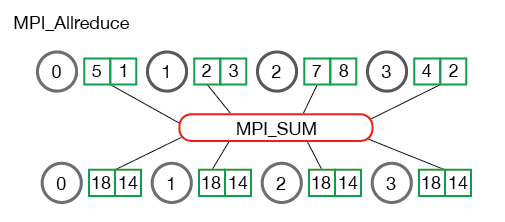
\includegraphics[width=10cm]{img.png}
  \caption{Example of All Reduce}
\end{figure}

After the all reduce takes place each parameter can be divided by n number of replicas in order to calculate the average, and then the local parameters can be updated. There are many method to to optimize the all reduce step such as using a ring all reduce algorithm. 

In order for each replica to be working at maximum efficiency they must finish calculating their gradients at the same time otherwise replicas can become idol.

\subsection{Bandwidth}
As most nodes will be run from homes and not data centres, wifi bandwidths will act as a large bottleeck to the training speed. The average internet speed in the U.S. is 189Mbps for download and 23Mbps for upload. Usually when AI is trained over multiple machines you can expect to see wired connection of speed upto 100s of Gbps.

So knowing this we have to come up with ways of reducing this effect of low bandwidths. The first option is to use a decentralized architecture is has been proved that a decentralized architectures handle better under low bandwidths

(https://proceedings.neurips.cc/paper/2017/file/f75526659f31040afeb61cb7133e4e6d-Paper.pdf)  

\subsection{Synchronism}

\subsection{Latency}

\bibliographystyle{plain}

\bibliography{reference}
\end{document}